\section{Iteratoren}
Iteratoren werden für das Iterieren über die Collectin s verwendet. Kriterien: Muss IEnumerable /IEnumberable<T> implementieren, Muss einer Implemtation von ähneln. $\rightarrow$ Mehtode GetEnumerator() mit Rückgabewert e, e hat eine Methode bool MoveNext(), e hat ein Property Current.

\subsection{Interfaces}
Es gibt zwei Interfaces, weil die ersten Varianten des .NET Frameworks keine Generics unterstützt haben. Sobald ein Generisches Interfaces implementiert wird, muss auch ein nicht generische implementiert werden.

\begin{lstlisting}
// Nicht generische Variante
public interface IEnumerable
{
	IEnumerator GetEnumerator();
}
public interface IEnumerator
{
	object Current { get; } 
	bool MoveNext(); 
	void Reset();
}
// Generische Variante
public interface IEnumerable<out T> : IEnumerable {
		IEnumerator<T> GetEnumerator();
}
public interface IEnumerator<out T> : IDisposable, IEnumerator {
	T Current { get; } 
	// Weitere Members werden vererbt
}
\end{lstlisting}

\subsection{Zugriff}
Mehrere aktive Iteratoren zur gleichen Zeit sind erlaubt. Enumerator-Objekt muss Zustand vollständig kapseln. So können unerwünschte Seiteneffekte unterbunden werden. Collection darf während der Iteration aber nicht verändert werden.

\subsection{Iterator-Methoden}
\subsubsection{yield return}
Gibt für den nächsten Wert für die nächste Iteration eines "foreach" Loops zurück.
\begin{lstlisting}
yield return "expression";
\end{lstlisting}

\subsection{Spezifische Iteratoren}
%TODO add iteratoren

\subsection{Extension Methode} %TODO move this chapter to the right place
Erlaubt das Erweitern bestehender Klassen um Methoden. Die Signatur der Klasse wird nicht verändert. Der Aufruf sieht jedoch so aus, als wäre es eine Methode der Klasse. \textit{Deklaration:} Muss in einer statischen Klasse deklariert sein, muss "static" sein, Erster Parameter mit "this" Schlüsselwort voranstehend.

\begin{lstlisting}
public static class ExtensionMethods {
	static string ToStringSafe(this object obj) {
		return obj == null
			? string.Empty : obj.ToString();
} 
public static void Test() {
	int myInt = 0; 
	object myObj = new object(); // Objects not null
	myInt.ToString(); 
	myInt.ToStringSafe(); 
	myObj.ToString(); 
	myObj.ToStringSafe(); // Object is null 
	myObj = null; myObj.ToString(); // Error
	myObj.ToStringSafe(); // Works
}
}

\end{lstlisting}

\subsection{Deferred Evaluation}
Werte werden erst dann berechnet, wenn sie abgefragt werden.
\pagebreak

% Week 07b
\section{Exceptions} 
Behandelt unerwartete Programmzustände oder Ausnahmeverhalten zur Laufzeit. Exceptions sollten so selten wie möglich und so oft wie nötig verwendet werden.  Möglichst konkrete Exception-Klassen verwenden. NIE über eine Web-Schnitstelle übermitteln!

Regeln: catch-Block wird sequenziell gesucht, Exception-Typ muss von System.Exception abgeleitet werden, finally-Block wird immmer ausgeführt.

Exceptions in C\# sind unchecked. Das bedeutet Aufrufer einer Methode müsssen die Exception nicht behandeln, wenn sie dies nicht wollen. Grosser Unterschied zu Java.

\begin{lstlisting}
FileStream s = null; 
try {
	s = new FileStream(@"C:\Temp\Test.txt", FileMode.Open);
} catch (FileNotFoundException e) {
		Console.WriteLine("{0} not found", e.FileName);
} catch (IOException) {
	Console.WriteLine("IO exception occurred");
} catch {
	Console.WriteLine("Unknown error occurred");
} finally {
	if (s != null) s.Close();
}
\end{lstlisting}

\subsection{Klasse System.Exception}
Ist die Basisklasse für alle Exceptions. Alle Exceptions müssen von der Klasse System.Exception ableiten. Besteht aus: Konstruktor und Properties. 

\textbf{Poperties}
\begin{itemize}
  \itemsep -0.5em 
  \item InnerException: Verschachtelte Exception
  \item Message: Fehlermeldung als String
  \item Source: Name der Applikation, Objekts, Frameworks, welches den Fehler verursacht hat
  \item StackTrace: Methodenaufrufkette als String
  \item TargetSite: Ausgeführter Code-Teil, der den Fehler verursacht
\end{itemize}


\begin{lstlisting}
public class Exception : ISerializable, _Exception {
	public Exception(); 
	public Exception(string message); 
	public Exception(string message, Exception innerException);
	public Exception InnerException { get; } 
	public virtual string Message { get; } 
	public virtual string Source { get; set; } 
	public virtual string StackTrace { get; } 
	public MethodBase TargetSite { get; }
	public override string ToString();
/* ... */
}
\end{lstlisting}

\subsection{Rethrowing}
Der Stack Trace bleibt erhalten, wenn das "throw" erneut ausgeführt wird.
\begin{lstlisting}
try {
	throw new Exception("Failure");
} catch (Exception e) {
	throw;
}
\end{lstlisting}

\subsection{Exception-Klassen}
\begin{figure}[h!]
	\centering
	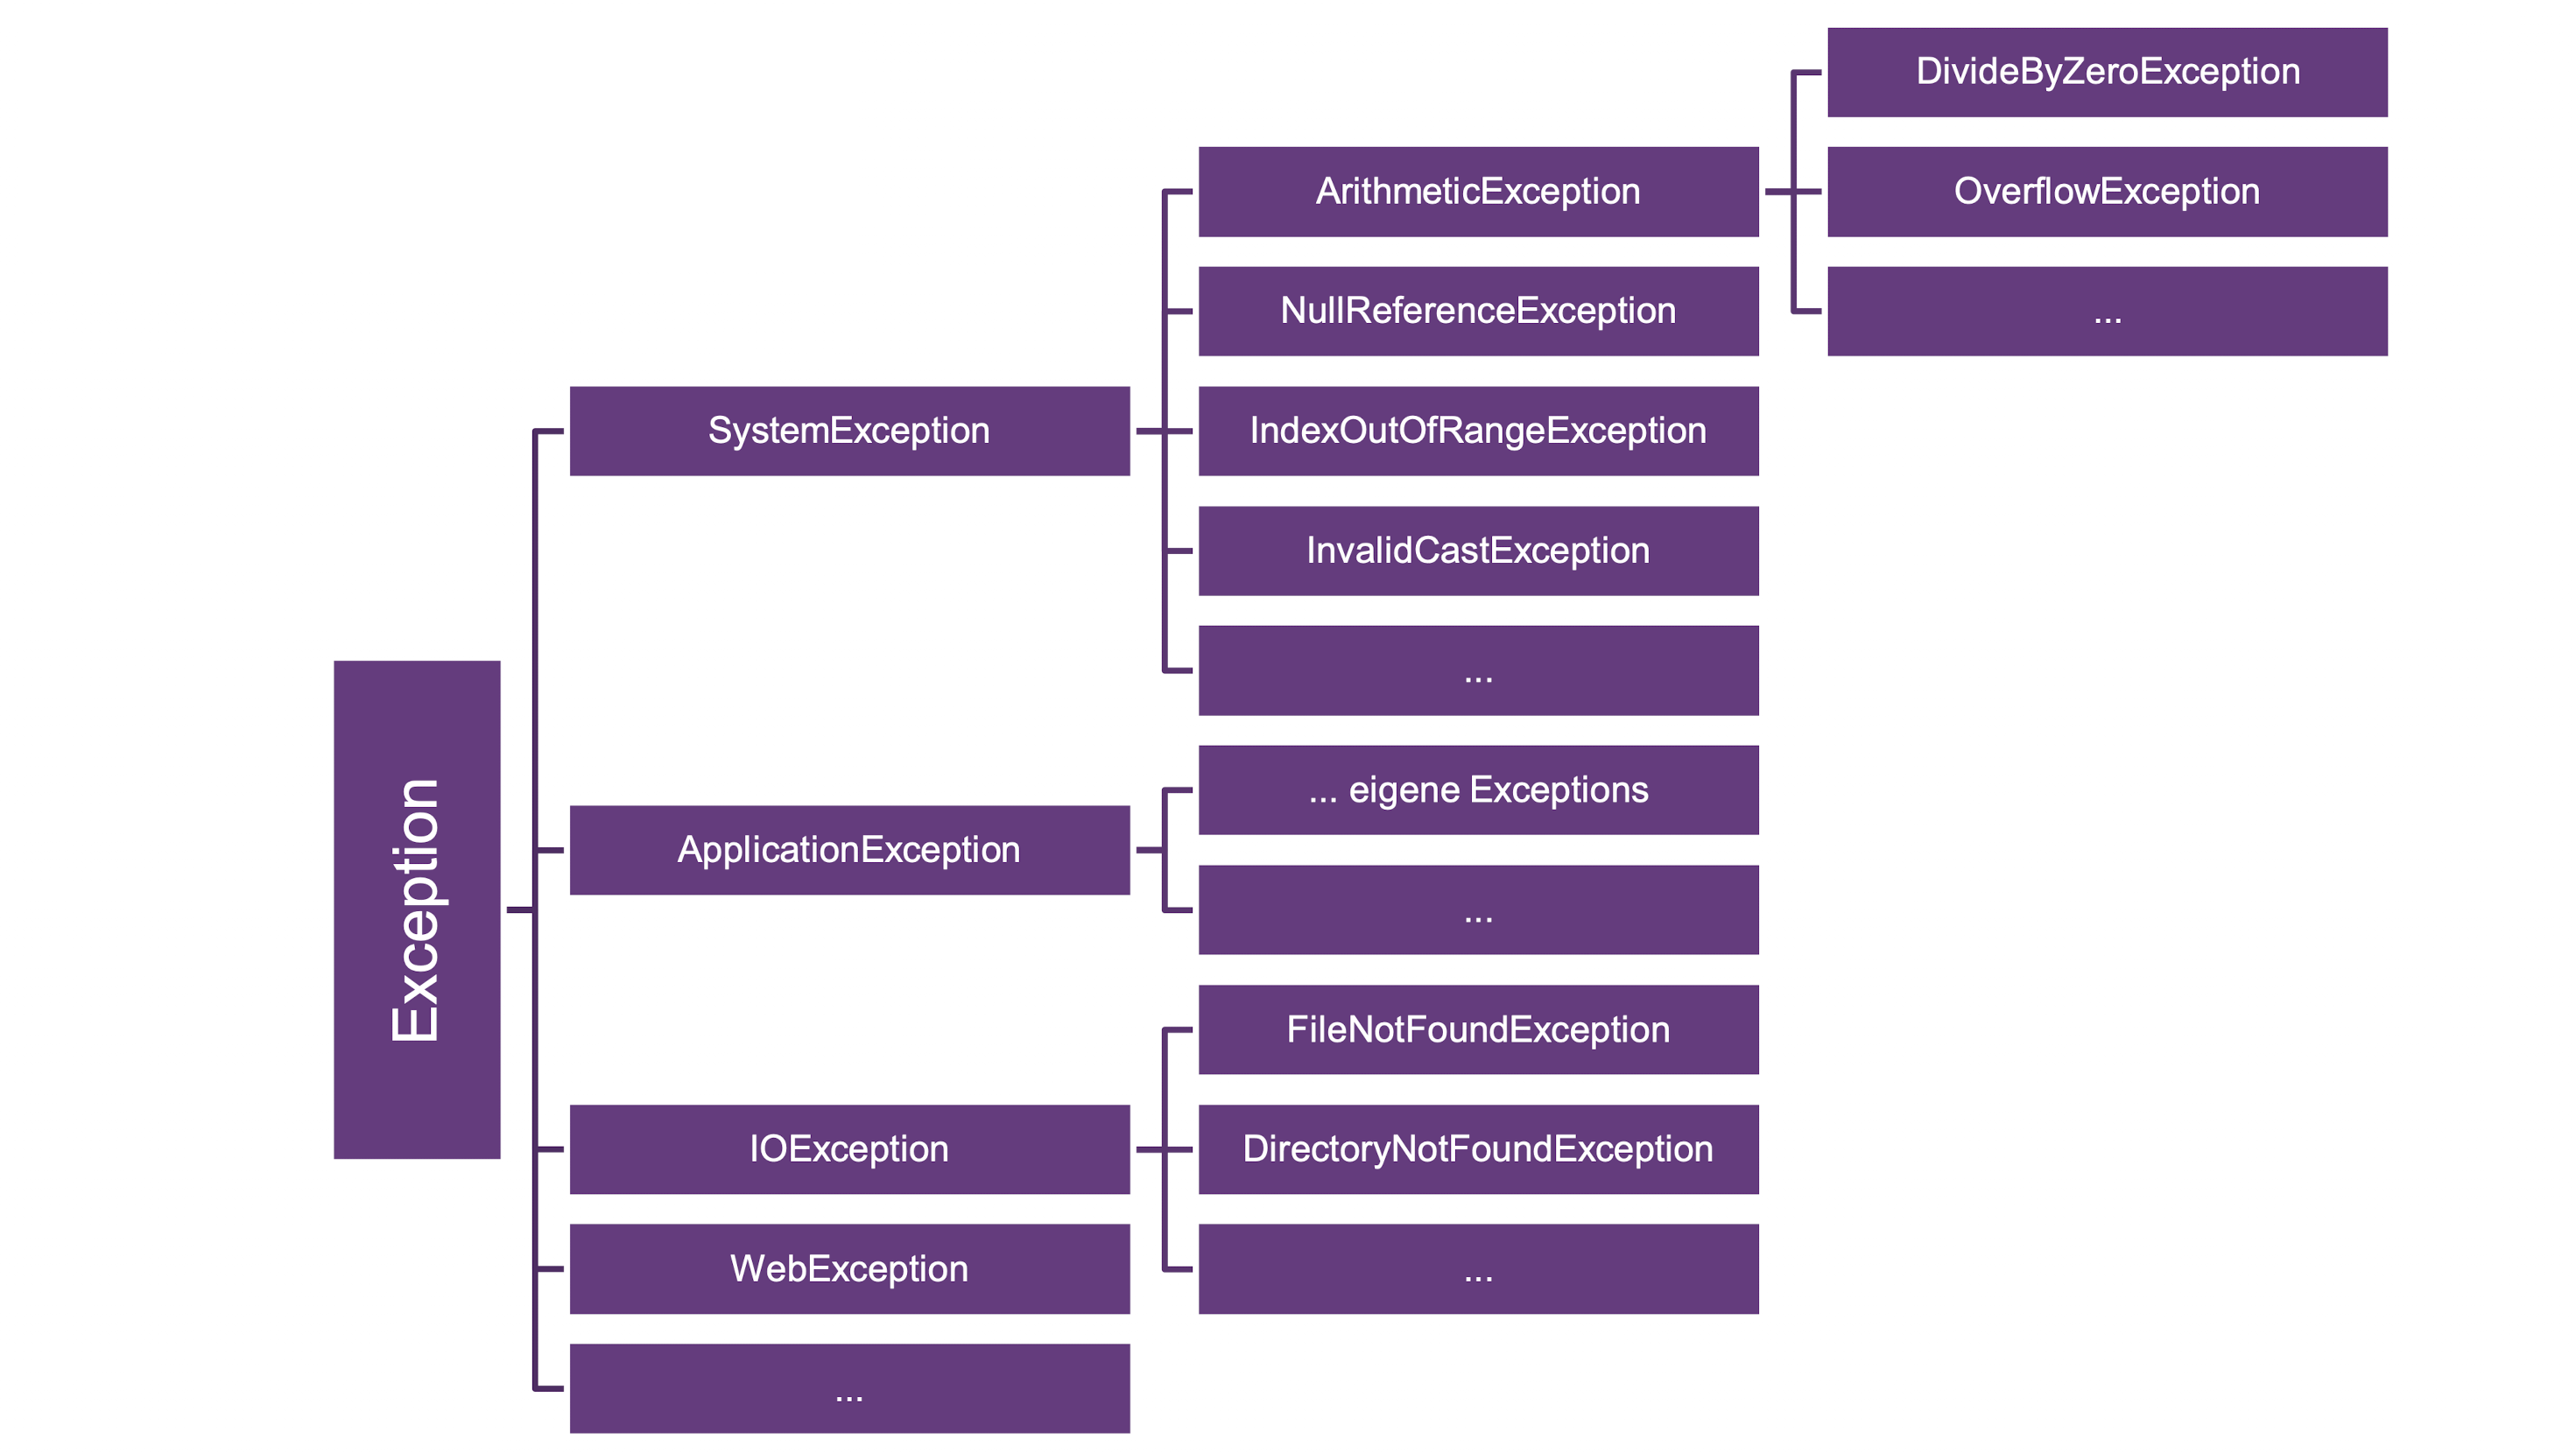
\includegraphics[width=0.75\linewidth]{exceptions}
  \caption{Exception-Typen}
\end{figure}

\subsection{Catch-Klausel}
Der Call Stack wird rückwärts nach passender "catch" Klausel durchsucht. Programmabbruch mit Fehlermeldung und Stack Trace, wenn keine "catch" Klausel gefunden wird.

\subsection{Exception Filters}
Catch-Block wird nur unter definierter Bedingung ausgeführt. Diese erwartet eine "bool" Expression.

\begin{lstlisting}
try {
} catch (Exception e) when (DateTime.Now.Hour < 18) {
} catch (Exception e) when (DateTime.Now.Hour >= 18) {
}
\end{lstlisting}

\pagebreak